\documentclass[tikz,border=4pt]{standalone}
\usepackage[T1]{fontenc}\usepackage{lmodern}\usepackage{xcolor}
\usepackage{tikz}

\definecolor{cI}{HTML}{EE7733}
\definecolor{cE}{HTML}{882255}
\definecolor{cR}{HTML}{0077BB}
\definecolor{cS}{HTML}{EE3377}
\definecolor{cM}{HTML}{33BBEE}
\definecolor{cO}{HTML}{BBBBBB}
\definecolor{eg}{HTML}{BDBDBD}

\begin{document}
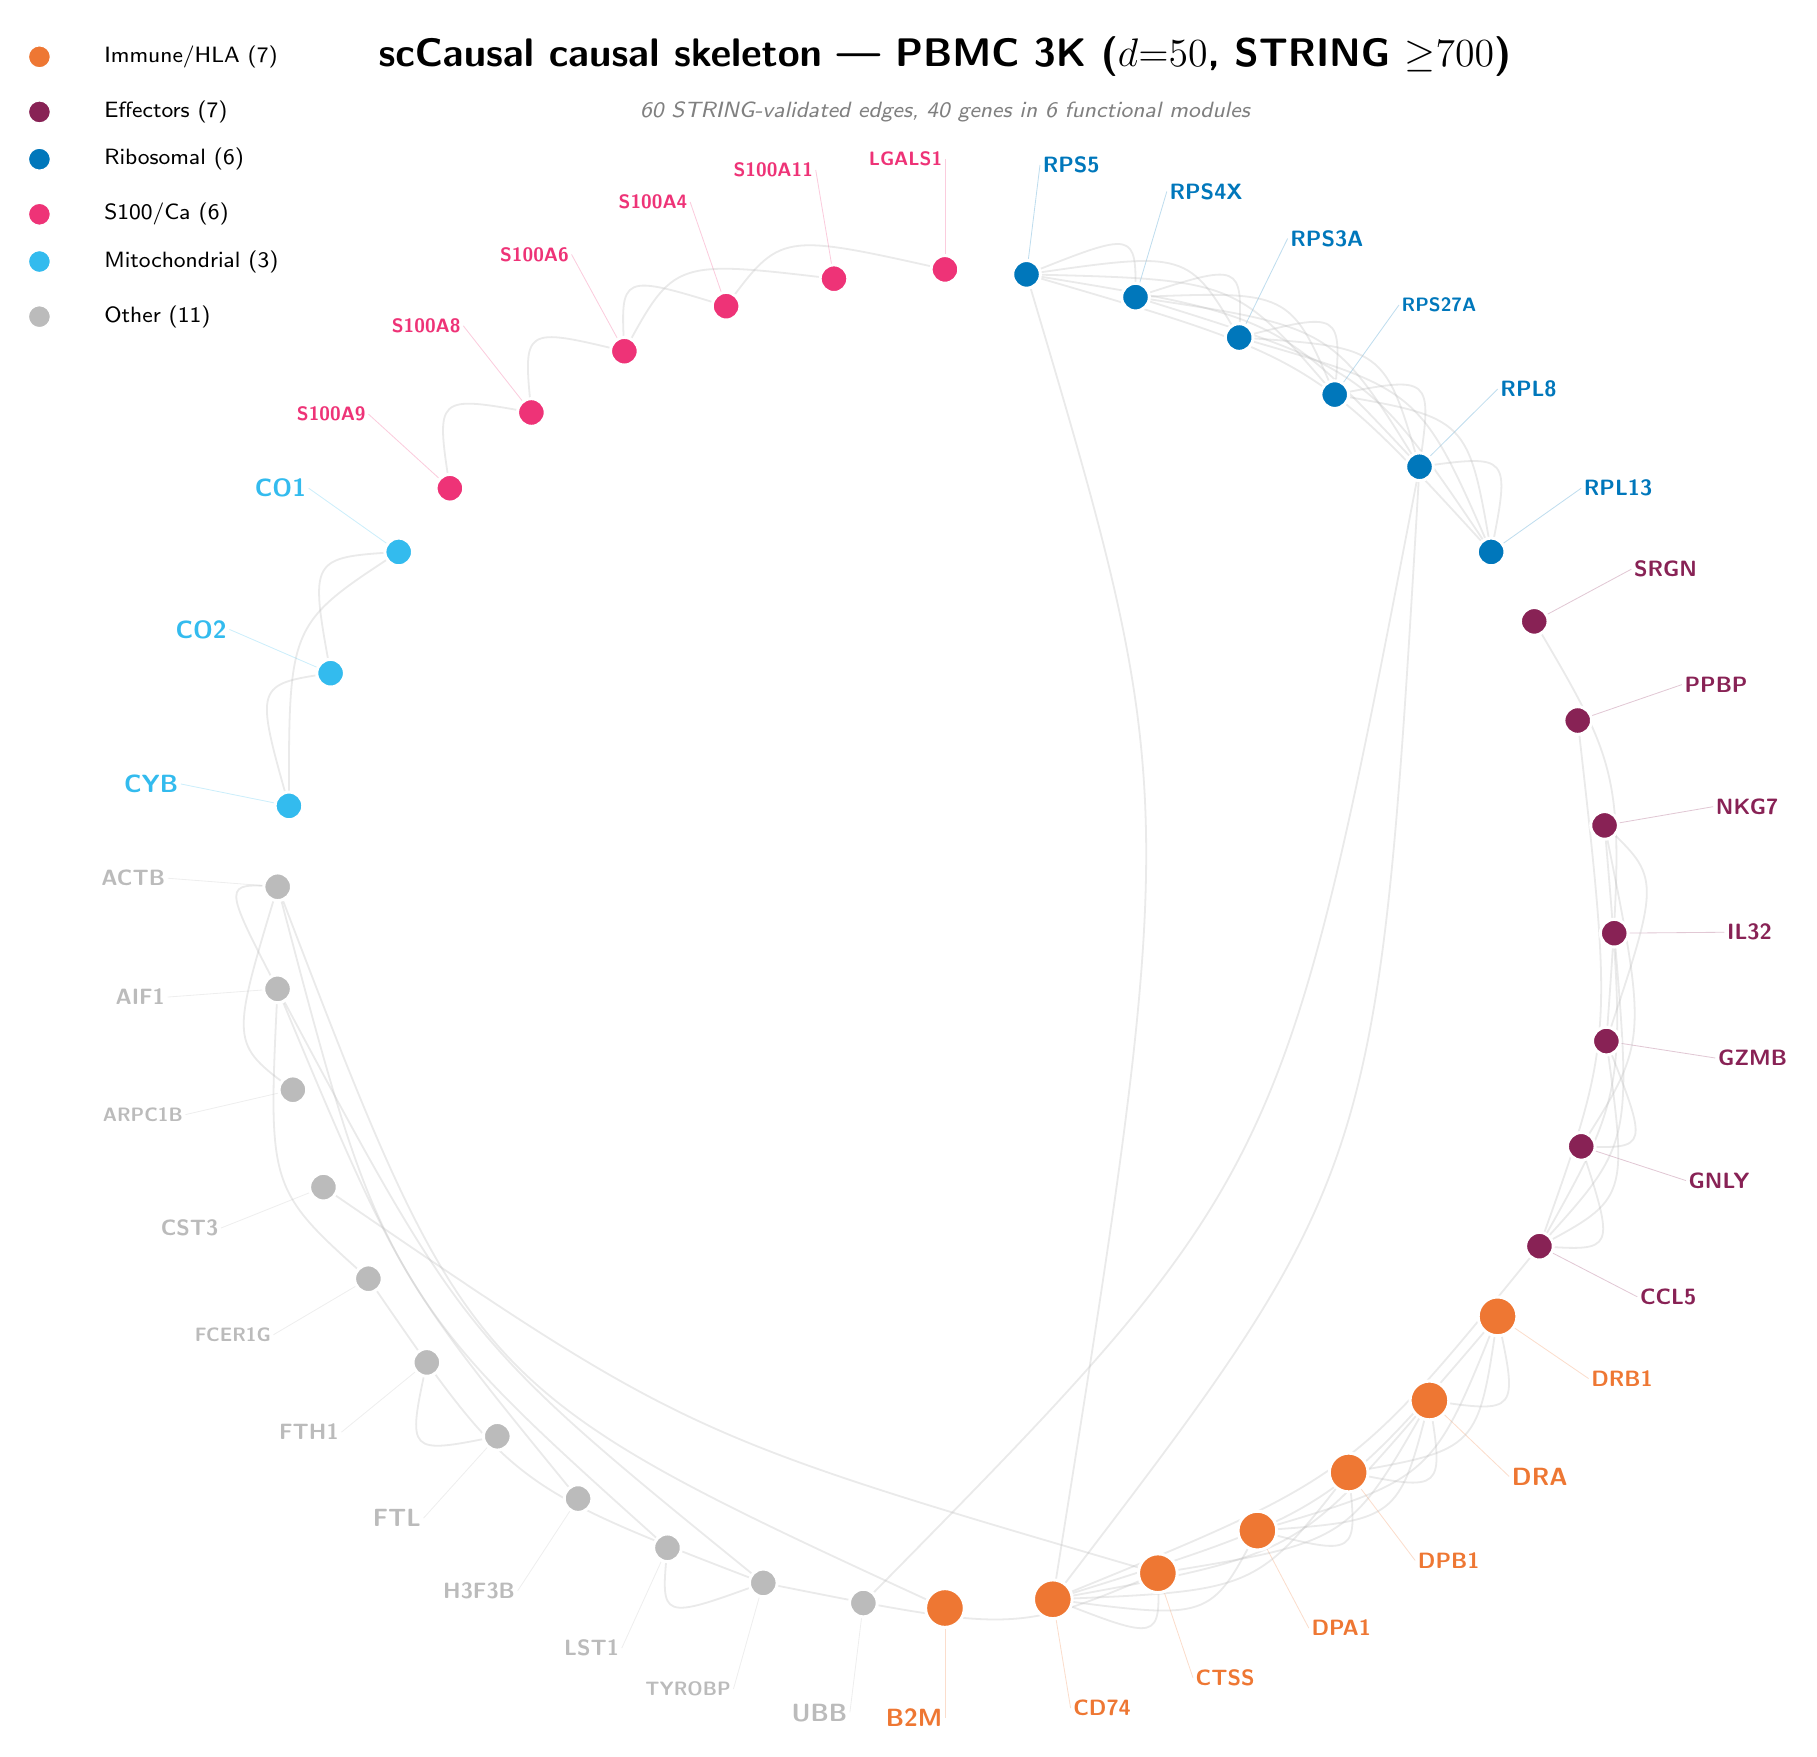
\begin{tikzpicture}[scale=1.0]

\node[font=\sffamily\bfseries\Large,align=center] at (0,11.2)
  {scCausal causal skeleton \textemdash\ PBMC 3K ($d{=}50$, STRING ${\geq}700$)};
\node[font=\sffamily\itshape\footnotesize,text=gray] at (0,10.5)
  {60 STRING-validated edges, 40 genes in 6 functional modules};

\draw[cI,line width=0.3pt,opacity=0.25] (0.000,-8.500) -- (0.000,-9.900);
\draw[cI,line width=0.3pt,opacity=0.25] (1.370,-8.389) -- (1.596,-9.771);
\draw[cI,line width=0.3pt,opacity=0.25] (2.704,-8.058) -- (3.150,-9.386);
\draw[cI,line width=0.3pt,opacity=0.25] (3.968,-7.517) -- (4.621,-8.755);
\draw[cI,line width=0.3pt,opacity=0.25] (5.127,-6.779) -- (5.972,-7.896);
\draw[cI,line width=0.3pt,opacity=0.25] (6.153,-5.864) -- (7.166,-6.830);
\draw[cI,line width=0.3pt,opacity=0.25] (7.018,-4.796) -- (8.174,-5.586);
\draw[cE,line width=0.3pt,opacity=0.25] (7.550,-3.905) -- (8.793,-4.548);
\draw[cE,line width=0.3pt,opacity=0.25] (8.081,-2.637) -- (9.411,-3.072);
\draw[cE,line width=0.3pt,opacity=0.25] (8.400,-1.300) -- (9.783,-1.515);
\draw[cE,line width=0.3pt,opacity=0.25] (8.500,0.070) -- (9.900,0.082);
\draw[cE,line width=0.3pt,opacity=0.25] (8.377,1.439) -- (9.757,1.677);
\draw[cE,line width=0.3pt,opacity=0.25] (8.036,2.771) -- (9.359,3.227);
\draw[cE,line width=0.3pt,opacity=0.25] (7.484,4.030) -- (8.717,4.693);
\draw[cR,line width=0.3pt,opacity=0.25] (6.937,4.912) -- (8.080,5.721);
\draw[cR,line width=0.3pt,opacity=0.25] (6.027,5.994) -- (7.020,6.981);
\draw[cR,line width=0.3pt,opacity=0.25] (4.950,6.910) -- (5.766,8.048);
\draw[cR,line width=0.3pt,opacity=0.25] (3.737,7.635) -- (4.352,8.892);
\draw[cR,line width=0.3pt,opacity=0.25] (2.420,8.148) -- (2.818,9.490);
\draw[cR,line width=0.3pt,opacity=0.25] (1.036,8.437) -- (1.207,9.826);
\draw[cS,line width=0.3pt,opacity=0.25] (0.000,8.500) -- (0.000,9.900);
\draw[cS,line width=0.3pt,opacity=0.25] (-1.409,8.382) -- (-1.641,9.763);
\draw[cS,line width=0.3pt,opacity=0.25] (-2.779,8.033) -- (-3.236,9.356);
\draw[cS,line width=0.3pt,opacity=0.25] (-4.071,7.461) -- (-4.742,8.690);
\draw[cS,line width=0.3pt,opacity=0.25] (-5.252,6.683) -- (-6.117,7.784);
\draw[cS,line width=0.3pt,opacity=0.25] (-6.287,5.721) -- (-7.322,6.663);
\draw[cM,line width=0.3pt,opacity=0.25] (-6.937,4.912) -- (-8.080,5.721);
\draw[cM,line width=0.3pt,opacity=0.25] (-7.802,3.372) -- (-9.087,3.928);
\draw[cM,line width=0.3pt,opacity=0.25] (-8.331,1.687) -- (-9.703,1.965);
\draw[cO,line width=0.3pt,opacity=0.25] (-8.474,0.660) -- (-9.870,0.768);
\draw[cO,line width=0.3pt,opacity=0.25] (-8.476,-0.637) -- (-9.872,-0.741);
\draw[cO,line width=0.3pt,opacity=0.25] (-8.281,-1.918) -- (-9.645,-2.234);
\draw[cO,line width=0.3pt,opacity=0.25] (-7.893,-3.155) -- (-9.193,-3.674);
\draw[cO,line width=0.3pt,opacity=0.25] (-7.322,-4.318) -- (-8.527,-5.029);
\draw[cO,line width=0.3pt,opacity=0.25] (-6.580,-5.381) -- (-7.664,-6.267);
\draw[cO,line width=0.3pt,opacity=0.25] (-5.685,-6.319) -- (-6.622,-7.359);
\draw[cO,line width=0.3pt,opacity=0.25] (-4.659,-7.110) -- (-5.426,-8.281);
\draw[cO,line width=0.3pt,opacity=0.25] (-3.524,-7.735) -- (-4.104,-9.009);
\draw[cO,line width=0.3pt,opacity=0.25] (-2.307,-8.181) -- (-2.686,-9.529);
\draw[cO,line width=0.3pt,opacity=0.25] (-1.036,-8.437) -- (-1.207,-9.826);

\draw[eg,line width=0.65pt,opacity=0.32] (-5.685,-6.319) .. controls (-6.833,-6.550) .. (-6.580,-5.381);
\draw[eg,line width=0.65pt,opacity=0.32] (0.000,-8.500) .. controls (-6.037,-5.720) .. (-8.474,0.660);
\draw[eg,line width=0.65pt,opacity=0.32] (-8.474,0.660) .. controls (-9.175,0.711) .. (-8.476,-0.637);
\draw[eg,line width=0.65pt,opacity=0.32] (-8.474,0.660) .. controls (-7.267,-3.925) .. (-4.659,-7.110);
\draw[eg,line width=0.65pt,opacity=0.32] (-8.474,0.660) .. controls (-9.078,-1.329) .. (-8.281,-1.918);
\draw[eg,line width=0.65pt,opacity=0.32] (6.937,4.912) .. controls (5.378,7.230) .. (2.420,8.148);
\draw[eg,line width=0.65pt,opacity=0.32] (6.937,4.912) .. controls (6.037,6.973) .. (3.737,7.635);
\draw[eg,line width=0.65pt,opacity=0.32] (6.937,4.912) .. controls (6.644,6.611) .. (4.950,6.910);
\draw[eg,line width=0.65pt,opacity=0.32] (6.937,4.912) .. controls (4.687,7.374) .. (1.036,8.437);
\draw[eg,line width=0.65pt,opacity=0.32] (6.937,4.912) .. controls (7.182,6.153) .. (6.027,5.994);
\draw[eg,line width=0.65pt,opacity=0.32] (-6.287,5.721) .. controls (-6.469,6.902) .. (-5.252,6.683);
\draw[eg,line width=0.65pt,opacity=0.32] (1.370,-8.389) .. controls (4.461,-7.827) .. (6.153,-5.864);
\draw[eg,line width=0.65pt,opacity=0.32] (1.370,-8.389) .. controls (3.003,1.824) .. (1.036,8.437);
\draw[eg,line width=0.65pt,opacity=0.32] (1.370,-8.389) .. controls (5.499,-2.998) .. (6.027,5.994);
\draw[eg,line width=0.65pt,opacity=0.32] (1.370,-8.389) .. controls (3.949,-8.284) .. (5.127,-6.779);
\draw[eg,line width=0.65pt,opacity=0.32] (1.370,-8.389) .. controls (3.369,-8.653) .. (3.968,-7.517);
\draw[eg,line width=0.65pt,opacity=0.32] (1.370,-8.389) .. controls (4.894,-7.292) .. (7.018,-4.796);
\draw[eg,line width=0.65pt,opacity=0.32] (1.370,-8.389) .. controls (5.160,-6.847) .. (7.550,-3.905);
\draw[eg,line width=0.65pt,opacity=0.32] (1.370,-8.389) .. controls (2.737,-8.924) .. (2.704,-8.058);
\draw[eg,line width=0.65pt,opacity=0.32] (6.153,-5.864) .. controls (6.340,-7.022) .. (5.127,-6.779);
\draw[eg,line width=0.65pt,opacity=0.32] (6.153,-5.864) .. controls (5.760,-7.391) .. (3.968,-7.517);
\draw[eg,line width=0.65pt,opacity=0.32] (6.153,-5.864) .. controls (7.285,-6.030) .. (7.018,-4.796);
\draw[eg,line width=0.65pt,opacity=0.32] (6.153,-5.864) .. controls (5.129,-7.661) .. (2.704,-8.058);
\draw[eg,line width=0.65pt,opacity=0.32] (-6.937,4.912) .. controls (-8.070,4.842) .. (-7.802,3.372);
\draw[eg,line width=0.65pt,opacity=0.32] (-6.937,4.912) .. controls (-8.334,4.000) .. (-8.331,1.687);
\draw[eg,line width=0.65pt,opacity=0.32] (-7.893,-3.155) .. controls (-3.294,-6.306) .. (2.704,-8.058);
\draw[eg,line width=0.65pt,opacity=0.32] (2.420,8.148) .. controls (3.778,8.591) .. (3.737,7.635);
\draw[eg,line width=0.65pt,opacity=0.32] (2.420,8.148) .. controls (4.385,8.229) .. (4.950,6.910);
\draw[eg,line width=0.65pt,opacity=0.32] (2.420,8.148) .. controls (2.428,8.992) .. (1.036,8.437);
\draw[eg,line width=0.65pt,opacity=0.32] (2.420,8.148) .. controls (4.923,7.771) .. (6.027,5.994);
\draw[eg,line width=0.65pt,opacity=0.32] (3.737,7.635) .. controls (5.044,7.972) .. (4.950,6.910);
\draw[eg,line width=0.65pt,opacity=0.32] (3.737,7.635) .. controls (3.086,8.736) .. (1.036,8.437);
\draw[eg,line width=0.65pt,opacity=0.32] (3.737,7.635) .. controls (5.582,7.514) .. (6.027,5.994);
\draw[eg,line width=0.65pt,opacity=0.32] (-2.779,8.033) .. controls (-4.125,8.447) .. (-4.071,7.461);
\draw[eg,line width=0.65pt,opacity=0.32] (-2.779,8.033) .. controls (-2.089,8.967) .. (0.000,8.500);
\draw[eg,line width=0.65pt,opacity=0.32] (4.950,6.910) .. controls (3.693,8.373) .. (1.036,8.437);
\draw[eg,line width=0.65pt,opacity=0.32] (4.950,6.910) .. controls (6.189,7.152) .. (6.027,5.994);
\draw[eg,line width=0.65pt,opacity=0.32] (-5.252,6.683) .. controls (-5.362,7.772) .. (-4.071,7.461);
\draw[eg,line width=0.65pt,opacity=0.32] (1.036,8.437) .. controls (4.232,7.915) .. (6.027,5.994);
\draw[eg,line width=0.65pt,opacity=0.32] (-7.802,3.372) .. controls (-8.767,3.230) .. (-8.331,1.687);
\draw[eg,line width=0.65pt,opacity=0.32] (6.027,5.994) .. controls (4.296,-3.022) .. (-1.036,-8.437);
\draw[eg,line width=0.65pt,opacity=0.32] (5.127,-6.779) .. controls (5.247,-7.848) .. (3.968,-7.517);
\draw[eg,line width=0.65pt,opacity=0.32] (5.127,-6.779) .. controls (6.772,-6.488) .. (7.018,-4.796);
\draw[eg,line width=0.65pt,opacity=0.32] (8.377,1.439) .. controls (8.929,-1.299) .. (8.081,-2.637);
\draw[eg,line width=0.65pt,opacity=0.32] (8.377,1.439) .. controls (8.664,-1.933) .. (7.550,-3.905);
\draw[eg,line width=0.65pt,opacity=0.32] (8.377,1.439) .. controls (9.089,0.770) .. (8.400,-1.300);
\draw[eg,line width=0.65pt,opacity=0.32] (8.081,-2.637) .. controls (8.515,-3.971) .. (7.550,-3.905);
\draw[eg,line width=0.65pt,opacity=0.32] (8.081,-2.637) .. controls (8.940,-2.669) .. (8.400,-1.300);
\draw[eg,line width=0.65pt,opacity=0.32] (-2.307,-8.181) .. controls (-3.615,-8.658) .. (-3.524,-7.735);
\draw[eg,line width=0.65pt,opacity=0.32] (-2.307,-8.181) .. controls (-6.091,-5.109) .. (-8.476,-0.637);
\draw[eg,line width=0.65pt,opacity=0.32] (-2.307,-8.181) .. controls (-5.514,-6.949) .. (-7.322,-4.318);
\draw[eg,line width=0.65pt,opacity=0.32] (-2.307,-8.181) .. controls (0.899,-8.820) .. (2.704,-8.058);
\draw[eg,line width=0.65pt,opacity=0.32] (3.968,-7.517) .. controls (6.193,-6.857) .. (7.018,-4.796);
\draw[eg,line width=0.65pt,opacity=0.32] (-4.071,7.461) .. controls (-3.440,8.622) .. (-1.409,8.382);
\draw[eg,line width=0.65pt,opacity=0.32] (-3.524,-7.735) .. controls (-6.700,-4.886) .. (-8.476,-0.637);
\draw[eg,line width=0.65pt,opacity=0.32] (7.550,-3.905) .. controls (8.725,-2.617) .. (8.500,0.070);
\draw[eg,line width=0.65pt,opacity=0.32] (7.550,-3.905) .. controls (8.675,-3.303) .. (8.400,-1.300);
\draw[eg,line width=0.65pt,opacity=0.32] (7.550,-3.905) .. controls (8.493,-1.267) .. (8.036,2.771);
\draw[eg,line width=0.65pt,opacity=0.32] (-8.476,-0.637) .. controls (-8.599,-3.177) .. (-7.322,-4.318);
\draw[eg,line width=0.65pt,opacity=0.32] (8.400,-1.300) .. controls (8.642,2.065) .. (7.484,4.030);

\fill[cI,draw=white,line width=1.1pt] (0.000,-8.500) circle (7pt);
\fill[cI,draw=white,line width=1.1pt] (1.370,-8.389) circle (7pt);
\fill[cI,draw=white,line width=1.1pt] (2.704,-8.058) circle (7pt);
\fill[cI,draw=white,line width=1.1pt] (3.968,-7.517) circle (7pt);
\fill[cI,draw=white,line width=1.1pt] (5.127,-6.779) circle (7pt);
\fill[cI,draw=white,line width=1.1pt] (6.153,-5.864) circle (7pt);
\fill[cI,draw=white,line width=1.1pt] (7.018,-4.796) circle (7pt);
\fill[cE,draw=white,line width=1.1pt] (7.550,-3.905) circle (5pt);
\fill[cE,draw=white,line width=1.1pt] (8.081,-2.637) circle (5pt);
\fill[cE,draw=white,line width=1.1pt] (8.400,-1.300) circle (5pt);
\fill[cE,draw=white,line width=1.1pt] (8.500,0.070) circle (5pt);
\fill[cE,draw=white,line width=1.1pt] (8.377,1.439) circle (5pt);
\fill[cE,draw=white,line width=1.1pt] (8.036,2.771) circle (5pt);
\fill[cE,draw=white,line width=1.1pt] (7.484,4.030) circle (5pt);
\fill[cR,draw=white,line width=1.1pt] (6.937,4.912) circle (5pt);
\fill[cR,draw=white,line width=1.1pt] (6.027,5.994) circle (5pt);
\fill[cR,draw=white,line width=1.1pt] (4.950,6.910) circle (5pt);
\fill[cR,draw=white,line width=1.1pt] (3.737,7.635) circle (5pt);
\fill[cR,draw=white,line width=1.1pt] (2.420,8.148) circle (5pt);
\fill[cR,draw=white,line width=1.1pt] (1.036,8.437) circle (5pt);
\fill[cS,draw=white,line width=1.1pt] (0.000,8.500) circle (5pt);
\fill[cS,draw=white,line width=1.1pt] (-1.409,8.382) circle (5pt);
\fill[cS,draw=white,line width=1.1pt] (-2.779,8.033) circle (5pt);
\fill[cS,draw=white,line width=1.1pt] (-4.071,7.461) circle (5pt);
\fill[cS,draw=white,line width=1.1pt] (-5.252,6.683) circle (5pt);
\fill[cS,draw=white,line width=1.1pt] (-6.287,5.721) circle (5pt);
\fill[cM,draw=white,line width=1.1pt] (-6.937,4.912) circle (5pt);
\fill[cM,draw=white,line width=1.1pt] (-7.802,3.372) circle (5pt);
\fill[cM,draw=white,line width=1.1pt] (-8.331,1.687) circle (5pt);
\fill[cO,draw=white,line width=1.1pt] (-8.474,0.660) circle (5pt);
\fill[cO,draw=white,line width=1.1pt] (-8.476,-0.637) circle (5pt);
\fill[cO,draw=white,line width=1.1pt] (-8.281,-1.918) circle (5pt);
\fill[cO,draw=white,line width=1.1pt] (-7.893,-3.155) circle (5pt);
\fill[cO,draw=white,line width=1.1pt] (-7.322,-4.318) circle (5pt);
\fill[cO,draw=white,line width=1.1pt] (-6.580,-5.381) circle (5pt);
\fill[cO,draw=white,line width=1.1pt] (-5.685,-6.319) circle (5pt);
\fill[cO,draw=white,line width=1.1pt] (-4.659,-7.110) circle (5pt);
\fill[cO,draw=white,line width=1.1pt] (-3.524,-7.735) circle (5pt);
\fill[cO,draw=white,line width=1.1pt] (-2.307,-8.181) circle (5pt);
\fill[cO,draw=white,line width=1.1pt] (-1.036,-8.437) circle (5pt);

\node[font=\sffamily\bfseries\small,text=cI,anchor=east,inner sep=0.8pt] at (0.000,-9.900) {B2M};
\node[font=\sffamily\bfseries\footnotesize,text=cI,anchor=west,inner sep=0.8pt] at (1.596,-9.771) {CD74};
\node[font=\sffamily\bfseries\footnotesize,text=cI,anchor=west,inner sep=0.8pt] at (3.150,-9.386) {CTSS};
\node[font=\sffamily\bfseries\footnotesize,text=cI,anchor=west,inner sep=0.8pt] at (4.621,-8.755) {DPA1};
\node[font=\sffamily\bfseries\footnotesize,text=cI,anchor=west,inner sep=0.8pt] at (5.972,-7.896) {DPB1};
\node[font=\sffamily\bfseries\small,text=cI,anchor=west,inner sep=0.8pt] at (7.166,-6.830) {DRA};
\node[font=\sffamily\bfseries\footnotesize,text=cI,anchor=west,inner sep=0.8pt] at (8.174,-5.586) {DRB1};
\node[font=\sffamily\bfseries\footnotesize,text=cE,anchor=west,inner sep=0.8pt] at (8.793,-4.548) {CCL5};
\node[font=\sffamily\bfseries\footnotesize,text=cE,anchor=west,inner sep=0.8pt] at (9.411,-3.072) {GNLY};
\node[font=\sffamily\bfseries\footnotesize,text=cE,anchor=west,inner sep=0.8pt] at (9.783,-1.515) {GZMB};
\node[font=\sffamily\bfseries\footnotesize,text=cE,anchor=west,inner sep=0.8pt] at (9.900,0.082) {IL32};
\node[font=\sffamily\bfseries\footnotesize,text=cE,anchor=west,inner sep=0.8pt] at (9.757,1.677) {NKG7};
\node[font=\sffamily\bfseries\footnotesize,text=cE,anchor=west,inner sep=0.8pt] at (9.359,3.227) {PPBP};
\node[font=\sffamily\bfseries\footnotesize,text=cE,anchor=west,inner sep=0.8pt] at (8.717,4.693) {SRGN};
\node[font=\sffamily\bfseries\footnotesize,text=cR,anchor=west,inner sep=0.8pt] at (8.080,5.721) {RPL13};
\node[font=\sffamily\bfseries\footnotesize,text=cR,anchor=west,inner sep=0.8pt] at (7.020,6.981) {RPL8};
\node[font=\sffamily\bfseries\fontsize{6.6}{7.6}\selectfont,text=cR,anchor=west,inner sep=0.8pt] at (5.766,8.048) {RPS27A};
\node[font=\sffamily\bfseries\footnotesize,text=cR,anchor=west,inner sep=0.8pt] at (4.352,8.892) {RPS3A};
\node[font=\sffamily\bfseries\footnotesize,text=cR,anchor=west,inner sep=0.8pt] at (2.818,9.490) {RPS4X};
\node[font=\sffamily\bfseries\footnotesize,text=cR,anchor=west,inner sep=0.8pt] at (1.207,9.826) {RPS5};
\node[font=\sffamily\bfseries\fontsize{6.6}{7.6}\selectfont,text=cS,anchor=east,inner sep=0.8pt] at (0.000,9.900) {LGALS1};
\node[font=\sffamily\bfseries\fontsize{6.6}{7.6}\selectfont,text=cS,anchor=east,inner sep=0.8pt] at (-1.641,9.763) {S100A11};
\node[font=\sffamily\bfseries\fontsize{6.6}{7.6}\selectfont,text=cS,anchor=east,inner sep=0.8pt] at (-3.236,9.356) {S100A4};
\node[font=\sffamily\bfseries\fontsize{6.6}{7.6}\selectfont,text=cS,anchor=east,inner sep=0.8pt] at (-4.742,8.690) {S100A6};
\node[font=\sffamily\bfseries\fontsize{6.6}{7.6}\selectfont,text=cS,anchor=east,inner sep=0.8pt] at (-6.117,7.784) {S100A8};
\node[font=\sffamily\bfseries\fontsize{6.6}{7.6}\selectfont,text=cS,anchor=east,inner sep=0.8pt] at (-7.322,6.663) {S100A9};
\node[font=\sffamily\bfseries\small,text=cM,anchor=east,inner sep=0.8pt] at (-8.080,5.721) {CO1};
\node[font=\sffamily\bfseries\small,text=cM,anchor=east,inner sep=0.8pt] at (-9.087,3.928) {CO2};
\node[font=\sffamily\bfseries\small,text=cM,anchor=east,inner sep=0.8pt] at (-9.703,1.965) {CYB};
\node[font=\sffamily\bfseries\footnotesize,text=cO,anchor=east,inner sep=0.8pt] at (-9.870,0.768) {ACTB};
\node[font=\sffamily\bfseries\footnotesize,text=cO,anchor=east,inner sep=0.8pt] at (-9.872,-0.741) {AIF1};
\node[font=\sffamily\bfseries\fontsize{6.6}{7.6}\selectfont,text=cO,anchor=east,inner sep=0.8pt] at (-9.645,-2.234) {ARPC1B};
\node[font=\sffamily\bfseries\footnotesize,text=cO,anchor=east,inner sep=0.8pt] at (-9.193,-3.674) {CST3};
\node[font=\sffamily\bfseries\fontsize{6.6}{7.6}\selectfont,text=cO,anchor=east,inner sep=0.8pt] at (-8.527,-5.029) {FCER1G};
\node[font=\sffamily\bfseries\footnotesize,text=cO,anchor=east,inner sep=0.8pt] at (-7.664,-6.267) {FTH1};
\node[font=\sffamily\bfseries\small,text=cO,anchor=east,inner sep=0.8pt] at (-6.622,-7.359) {FTL};
\node[font=\sffamily\bfseries\footnotesize,text=cO,anchor=east,inner sep=0.8pt] at (-5.426,-8.281) {H3F3B};
\node[font=\sffamily\bfseries\footnotesize,text=cO,anchor=east,inner sep=0.8pt] at (-4.104,-9.009) {LST1};
\node[font=\sffamily\bfseries\fontsize{6.6}{7.6}\selectfont,text=cO,anchor=east,inner sep=0.8pt] at (-2.686,-9.529) {TYROBP};
\node[font=\sffamily\bfseries\small,text=cO,anchor=east,inner sep=0.8pt] at (-1.207,-9.826) {UBB};

\fill[cI,draw=white,line width=0.5pt] (-11.5,11.2) circle (4pt);
\node[font=\sffamily\footnotesize,anchor=west] at (-10.8,11.2) {Immune/HLA (7)};
\fill[cE,draw=white,line width=0.5pt] (-11.5,10.5) circle (4pt);
\node[font=\sffamily\footnotesize,anchor=west] at (-10.8,10.5) {Effectors (7)};
\fill[cR,draw=white,line width=0.5pt] (-11.5,9.9) circle (4pt);
\node[font=\sffamily\footnotesize,anchor=west] at (-10.8,9.9) {Ribosomal (6)};
\fill[cS,draw=white,line width=0.5pt] (-11.5,9.2) circle (4pt);
\node[font=\sffamily\footnotesize,anchor=west] at (-10.8,9.2) {S100/Ca (6)};
\fill[cM,draw=white,line width=0.5pt] (-11.5,8.6) circle (4pt);
\node[font=\sffamily\footnotesize,anchor=west] at (-10.8,8.6) {Mitochondrial (3)};
\fill[cO,draw=white,line width=0.5pt] (-11.5,7.9) circle (4pt);
\node[font=\sffamily\footnotesize,anchor=west] at (-10.8,7.9) {Other (11)};
\end{tikzpicture}
\end{document}
